% All content is copyright 2023, 2024 the authors.

% To-Do
% -----
% - Hogg & Kate: read Oayda et al. 2024. do we agree with their claims about the ability to measure the dipole from a small footprint / masked skies ?


\documentclass[modern]{aastex631}
\usepackage[utf8]{inputenc}
\usepackage{amsmath}
\usepackage{xspace}
\usepackage{graphicx}
\usepackage{bm}
\usepackage{comment}

\setlength{\parindent}{3.5ex}
\sloppy\sloppypar\raggedbottom\frenchspacing

% commands
\newcommand{\abby}[1]{\textbf{Abby says: #1}}
\newcommand{\choice}[1]{\textcolor{teal}{#1}}
\newcommand{\ksf}[1]{\textcolor{purple}{KSF says: #1}}
\newcommand{\catwise}{\textsl{CatWISE}\xspace}
\newcommand{\catwisetwentytwenty}{\textsl{CatWISE2020}\xspace}
\newcommand{\quaia}{\textsl{Quaia}\xspace}
\newcommand{\gaia}{\textsl{Gaia}\xspace}
\newcommand{\wise}{\textsl{WISE}\xspace}
\newcommand{\unwise}{\textsl{unWISE}\xspace}
\newcommand{\vobs}{\boldsymbol{v}_0}
\newcommand{\dd}{\mathrm{d}}
\newcommand{\Cinv}{\boldsymbol{C}^{-1}}
\newcommand{\w}{\mathrm{W}}
\newcommand{\g}{\mathrm{G}}
\newcommand{\npix}{n_\mathrm{pix}}
\newcommand{\nside}{N_\mathrm{side}}
\newcommand{\dipamp}{|\vec{\mathcal{D}}_k|}

\begin{document}

\title{Cosmic isotropy and the quasar dipole:\\
Anomalous power on large angular scales}
\author[0000-0001-6069-5383]{Abby E. Williams}
\affiliation{Department of Physics, The University of Chicago, 5640 South Ellis Avenue, Chicago, IL 606137, USA}

\author[0000-0001-8764-7103]{Kate Storey-Fisher}
\affiliation{Donostia International Physics Center, Manuel Lardizabal Ibilbidea, 4, 20018 Donostia, Gipuzkoa, Spain}

\author[0000-0003-2866-9403]{David W. Hogg}
\affiliation{Center for Cosmology and Particle Physics, Department of Physics, New York University, 726 Broadway, New York, NY 10003, USA}
\affiliation{Center for Computational Astrophysics, Flatiron Institute, 162 Fifth Avenue, New York, NY
10010, USA}
\affiliation{Max Planck Institute for Astronomy, K{\"o}nigstuhl 17, 69117 Heidelberg, Germany}

\begin{abstract}\noindent % Hogg insists on this
    There is a discrepancy in amplitude between the dipole measured in the cosmic microwave background and the dipole measured in the distribution of radio and infrared selected quasars.
    These dipoles should be consistent if they are both caused primarily by a local Doppler boost.
    Here we investigate the amplitudes of the large angular-scale spherical harmonic modes ($1\leq\ell\leq 8$) in the sky distribution of two all-sky quasar catalogs, \quaia and \catwise, both of which depend on NASA\! \wise infrared data.
    We adopt a forward-modeling approach to generate all-sky mock density maps for both catalogs and employ a form of simulation-based \abby{Hogg: field-level?} inference to simultaneously measure the dipole amplitude and the level of any excess power on these large angular scales.
    This inference yields dipole amplitude $X^{+Y}_{-Z}$ in the direction of the kinematic expectation (xx sigma higher than the expected amplitude) and an excess angular power variance amplitude of $X^{+Y}_{-Z}$.
    The excess power we find could indicate a very severe problem with the $\Lambda$CDM model.
    Our view instead is that this power is probably produced by unmodeled selection effects in these two quasar catalogs, and that it is contaminating all quasar dipole measurements that do not account for it.
\end{abstract}

\keywords{foo --- bar}

\section{Introduction}
Our peculiar velocity relative to the rest frame of the Universe creates a dipole in the signals we measure across the sky.
There exists a dipole in the temperature of the CMB, taken to be purely kinematic in origin, which is used to infer a heliocentric velocity of
\begin{equation}
    \label{eq:CMB_velocity}
    v_0 = (369.825\pm 0.070)\,\mathrm{km\, s}^{-1}\ \mathrm{towards}\ (l,b) = (264.021\pm0.009^\circ, 48.253\pm0.004^\circ)
\end{equation}
\citep{planck_collaboration_planck_2020}.
This Doppler boost of the CMB monopole is so well-measured by Planck that its expected modulations and aberrations of the temperature fluctuations have been detected in the CMB spectrum \citep{planck_collaboration_planck_2014}.

The CMB and LSS rest frames should converge under the standard $\Lambda$CDM model; the kinematic dipole anisotropy in the number count of LSS tracers should align with the CMB temperature dipole in direction, with its amplitude modified by a prefactor that depends on the tracer sample.
The predominant approximation comes from \citet{ellis_expected_1984} and gives the expected kinematic dipole from LSS as
\begin{equation}
    \label{eq:ellisbaldwin}
    \vec{\mathcal{D}} \simeq \left[2+x(1+\alpha)\right]\vobs/c
\end{equation}
where $x$ is the number-count slope of the sources at the magnitude limit of the sample, and $\alpha$ is the effective spectral index \abby{Hogg/KSF: will the average reader know what effective spectral index means, or should I define?} of the sources.

However, there is a claimed \abby{Hogg/KSF: help with word choice here?} tension between these two dipole measurements.
Several initial analyses were performed on radio source counts from the 1.4 GHz NRAO VLA Sky Survey (NVSS; \citealt{condon_nrao_1998}).
Though \citet{blake_detection_2002} found this matter dipole to be broadly consistent with the expectation from the CMB, later work such as \citet{singal_large_2011} showed that while the direction of the dipole roughly agreed with the CMB, its amplitude was larger than expected from Eq. \ref{eq:ellisbaldwin}.
Results remain mixed; for example, \citet{darling_universe_2022} found the matter dipole to be consistent with the CMB expectation in both direction and amplitude using radio data from the Very Large Array Sky Survey (VLASS; \citealt{lacy_karl_2020}) and the Rapid
Australian Square Kilometer Array Pathfinder Continuum
Survey (RACS; \citealt{mcconnell_rapid_2020}).

Recently, \citet{secrest_test_2021} (hereafter S21) measured the dipole from a sample of infrared-selected quasars from \catwisetwentytwenty to have more than twice the expected amplitude at $4.9\sigma$ confidence.
\citet{dam_testing_2022} confirmed the S21 result for the identical sample using a different, Bayesian approach.
This suggests that the source of the discrepancy with the CMB dipole is the sample itself (with the specific choices made in its construction) rather than the analysis method.
\abby{should add more recent paper results at this point...}

Importantly, unmitigated systematics in the source density maps would impact the angular power at several modes, not just $\ell=1$, though investigations of the angular power in these maps at large angular scales ($\ell\lesssim 10$) have been rare.
\abby{``rare"... back this up with citations!}

\quaia, a more recent all-sky spectroscopic quasar sample constructed from \gaia and \unwise, offers a new opportunity to measure the LSS dipole \citep{storey-fisher_quaia_2023}.
The catalog is not totally independent from the S21 sample, since both rely on infrared observations from \textit{WISE}—nevertheless, \quaia involves different observations, source selection, and systematics, and therefore can serve as a check on the dipole measured in S21.
In this work, we measure the number-count dipole in the S21 and \quaia samples using the approach described in S21 and compare each to their expectation: the direction of the CMB dipole with amplitude given by Eq. \ref{eq:ellisbaldwin}.
However, in order to avoid mode-coupling effects on the measured dipole, we further employ a forward-modeling approach to infer both the amplitude of the dipole in the expected direction and the overall level of excess angular power at multipoles $\ell\le 8$.
\abby{need to explain motivation: why are we doing this? If there is unaccounted-for angular power at other large angular scales, due to mode coupling this could inflate the measured dipole amplitude on the cut sky... (I'm actually not sure how much I trust this statement now since checking out \citet{oayda_cosmic_2024}...)}
We generate mock all-sky quasar density maps with the same selection function as applied to the real data and employ an Approximate Bayesian Computation (ABC) scheme to estimate the parameter posteriors.

This paper is organized as follows.
Section \ref{sec:data} describes the construction of the all-sky samples from \catwise and \quaia.
Section \ref{sec:dipole_theory} discusses the theoretical matter dipole and the expected amplitude of the dipole in the \catwise and \quaia catalogs under the Ellis-Baldwin approximation.
In Section \ref{sec:inference_method} we present our forward-modeling approach, the quasar density model used to generate mock sky maps, and parameter inference via Approximate Bayesian Computation (ABC) using a Sequential Monte Carlo method.
Finally, Sections \ref{sec:results} and \ref{sec:discussion} respectively contain the results and subsequent discussion.


\section{The all-sky quasar samples}
\label{sec:data}

Here we describe the construction of two all-sky quasar samples, the \catwise sample used in S21, and the new \quaia sample.

\subsection{The CatWISE2020 Quasar Sample}
\label{sec:catwise}
The S21 quasar sample was constructed from \catwisetwentytwenty, an all-sky infrared catalog constructed from \wise and NEOWISE \citep{marocco_catwise2020_2021}.
The number-count dipole was measured from a final sample of 1,355,352 quasars, shown in Figure \ref{fig:S21_map}.
Here we summarize the steps used in \citet{secrest_test_2021} to construct the sample.

First, to select AGNs, we make a color cut in the initial sources from \catwisetwentytwenty of $\w 1-\w 2\geq0.8$.
The W1 and W2 magnitudes are corrected for galactic reddening using the \citet{planck_collaboration_planck_2014} dust map and extinction coefficients from \citet{wang_optical_2019} (Table 3): total-to-selective extinction ratio $R_V=3.1$, and for the \wise bands, relative extinction ratios $R\w 1=0.039\pm 0.004$ and $R\w 2=0.026\pm 0.004$.
Next, we make the magnitude cut $9\leq\w 1\leq 16.4$. According to S21, beyond $\w 1=16.4$ source density becomes uneven due to \wise's ecliptic scan pattern, and $\w 1=9$ was selected as a lower bound to avoid potential saturation.
To reduce contamination from stars and dust, we make a cut in absolute galactic latitude $\vert b\vert > 30^\circ$.
% This is the fiducial galactic plane cut; see Section \ref{sec:dipole} for an investigation of how other values impact the measured dipole.
To reduce contamination from spurious sources, we also mask several smaller regions: the MCs, bright galaxies from 2MASS, bright artifacts from \wise, and other areas of low completeness.
There are 291 total masked regions.
At this point we convert the list of sources into a healpix map of source densities with $N_\mathrm{side}=64$ \citep{gorski_healpix_2005}.
Note that if any sources in a healpixel are masked, the entire healpixel gets masked.
Finally, S21 noticed a mild inverse linear trend in source density with absolute ecliptic latitude.
Assuming that there is no true correlation between source density and ecliptic latitude (i.e. that the observed trend is a residual systematic), they fit a slope to the absolute sine of ecliptic latitude and correct the source counts by this slope.
We perform this last step when replicating S21's dipole measurement.
However, unless otherwise stated, in other analyses we forego the ecliptic latitude density correction and instead correct the source counts using a selection function map (see Section \ref{sec:selfuncs}).

\begin{figure}
    \centering
    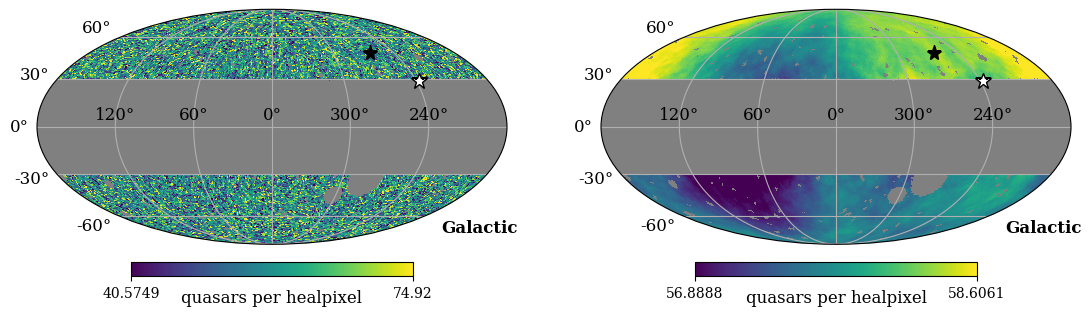
\includegraphics[width=\textwidth]{images/catwise_map.png}
    \caption{Healpix density maps ($\nside=64$) of the S21 sample in galactic coordinates using a Mollweide projection. The fiducial sample contains a $|b|>30^\circ$ plane cut as well as smaller masks. The black star marks the direction of the CMB dipole, and the white star marks the direction of the dipole measured in this sample via the standard method (see Section \ref{sec:standard_dipole}). \textit{Left:} Source counts in each healpixel. The color bar spans the monopole $\pm$ twice the standard deviation of the map. \textit{Right:} Source counts smoothed to 1 steradian, with the color bar centered at the monopole.}
    \label{fig:S21_map}
\end{figure}


\subsection{The Quaia Quasar Sample}
\label{sec:quaia}
The \gaia-\unwise Quasar Catalog, or \quaia, is an all-sky spectroscopic catalog constructed from quasar candidates in \gaia DR3 and infrared observations from \wise \citep{storey-fisher_quaia_2023}.
It spans the largest comoving volume of any existing quasar catalog \abby{KSF: is this still true?}, making it especially suited for large-scale precision cosmological measurements.
We use the $G\leq 20.0$ catalog as our fiducial sample, which has 530,364 sources in the fiducial $|b|<30^\circ$ cut, shown in Figure \ref{fig:quaia_map}.
% We also use the less pure $G\leq 20.5$ sample when exploring dependence on magnitude limit.

The construction of the \quaia sample is largely analogous to the S21 method.
\abby{KSF: justification for why we don't (need to) correct the magnitudes for reddening like in S21?}
The masks are identical, but we make magnitude cuts in the optical G band ($\mathrm{G}\leq 20.0$) rather than the infrared W1 band.
We also correct the source counts with \quaia's selection function (see Section \ref{sec:selfuncs}).
Figure \ref{fig:quaia_map} shows the \quaia sample after correcting by the selection function.

\begin{figure}
    \centering
    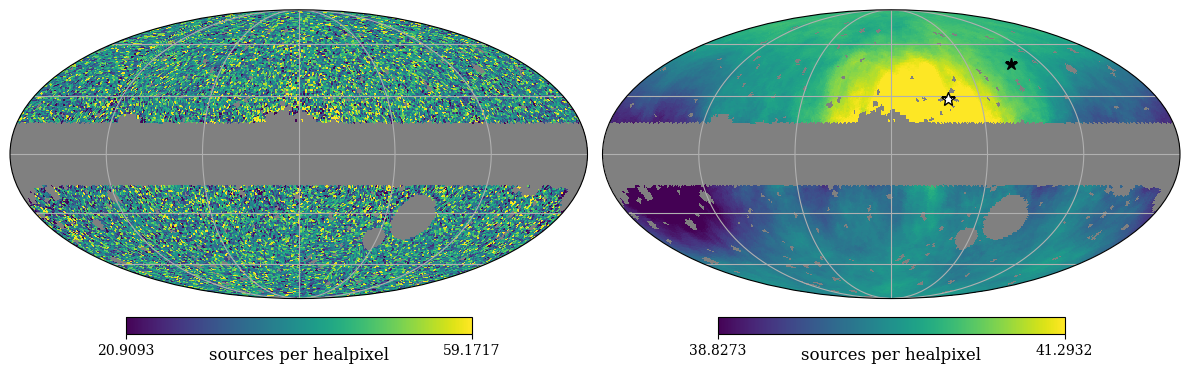
\includegraphics[width=\textwidth]{images/quaia_map.png}
    \caption{Healpix density maps ($\nside=64$) of the \quaia sample in galactic coordinates using a Mollweide projection. The fiducial sample contains a $|b|>30^\circ$ plane cut as well as smaller masks. The black star marks the direction of the CMB dipole, and the white star marks the direction of the dipole measured in this sample via the standard method (see Section \ref{sec:standard_dipole}). \textit{Left:} Source counts in each healpixel. The color bar spans the monopole $\pm$ twice the standard deviation of the map. \textit{Right:} Source counts smoothed to 1 steradian, with the color bar centered at the monopole.}
    \label{fig:quaia_map}
\end{figure}


\subsection{Selection functions}
\label{sec:selfuncs}
For each sample, we generate a selection function, which gives the completeness in each pixel relative to the predicted number of quasars that would be observed in the absence of any selection effects.
To model the selection function, \cite{storey-fisher_quaia_2023} uses a Gaussian process to fit healpix maps ($\nside=64$; \citealt{gorski_healpix_2005}) of the systematics templates to the source counts in each healpixel.
The systematics templates for \quaia are dust extinction, \gaia and \unwise source density, and those missions' scanning laws.\abby{might want to be more specific ?}
We apply the same procedure to \catwise, using the \unwise source density and zodiacal light as the templates.
To correct the observed counts by the selection function, we simply divide the counts by the relative completeness in each pixel.
Figure \ref{fig:selfuncs} shows the selection function maps generated for each quasar sample.

\begin{figure}
    \centering
    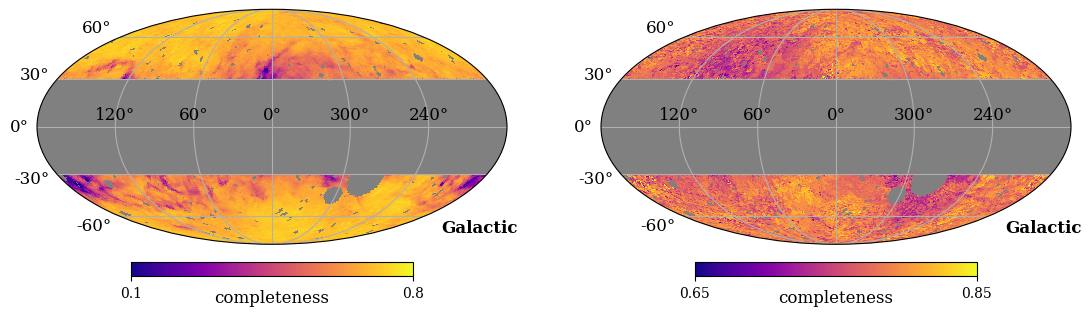
\includegraphics[width=\textwidth]{images/selfuncs.png}
    \caption{Selection function maps ($\nside=64$) for the \quaia $G\le20.0$ (\textit{left}) and \catwisetwentytwenty (\textit{right}) quasar catalogs.}
    \label{fig:selfuncs}
\end{figure}


\section{The number-count dipole}
\label{sec:dipole_theory}

\subsection{The Ellis-Baldwin approximation}
\label{sec:EB}
Under the kinematic interpretation of the dipole, both the CMB and matter dipole anisotropies are caused by our proper motion with respect to the frame in which the CMB is maximally isotropic.
Therefore the expected direction of the matter dipole is the same as the CMB dipole (Eq. \ref{eq:CMB_velocity}).
The expected amplitude of the matter dipole, however, depends on the velocity $\vobs$ of the observer and the properties of the sources in the sample, in particular the number-count slope $x$ and the effective spectral index $\alpha$ of the sample.
Eq. \ref{eq:ellisbaldwin} is the result of two special relativistic effects: there is an abberration effect causing sources in direction $\hat{v}_0$ to appear closer together, and there is a flux effect causing sources in direction $\hat{v}_0$ to appear brighter.
These effects result in additional dependencies on $x$, the slope of the number of sources at the magnitude limit of the sample, and $\alpha$, the effective spectral index of the sample.
As described in \citet{ellis_expected_1984}, both of these values come in at roughly order unity.

We calculate $x$ using
\begin{equation}
    x \equiv -\left.\frac{\dd\ln N(>S_\nu)}{\dd\ln S_\nu}\right|_{S_\mathrm{min}} ~,
\end{equation}
where $S_\nu$ is the flux density, $N(>S_\nu)$ is the number of sources above a given flux density limit, and $S_\mathrm{min}$ is the flux-density limit of the sample.
The results for both samples are shown in Figure \ref{fig:alphas_xs}.
For \catwise, the number-count slope at the fiducial magnitude limit $\w 1=16.4$ is $x=1.75$.
For \quaia, the number-count slope at the fiducial magnitude limit $\g =20.0$ is $x=1.30$.

To calculate $\alpha$, we assume that the flux density of each source roughly follows a power law, $S_\nu(\nu)\sim\nu^{-\alpha}$.
We can estimate $\alpha$ for any source with flux measurements at two or more frequencies.
If we have magnitudes of the source in two spectral bands, $m_1$ and $m_2$ in the AB system, from the definition of magnitude they are related to flux by
\begin{equation}
    (m_1-m_2)_\mathrm{AB}=-2.5(\log S_{\nu,m_1}-\log S_{\nu,m_2}) ~,
\end{equation}
where $S_{\nu}$ is the flux density (units of W m$^{-2}$ Hz$^{-1}$).
Since magnitudes in the AB system are defined relative to a source with flat spectrum, $\nu S_\nu=$ constant, $\alpha$ can be computed from the slope of the AB magnitudes,
\begin{equation}
    \alpha = -\frac{\dd\log S_\nu}{\dd\log\nu} \approx -\frac{\log S_{\nu,m_1}-\log S_{\nu,m_2}}{\log\left(\nu_{m_1}/\nu_{m_2}\right)} = -\frac{1}{2.5}\frac{(m_1-m_2)_{\mathrm{AB}}}{\log(\lambda_{m_2}/\lambda_{m_1})} ~,
\end{equation}
where $\lambda$ is the wavelength, $\lambda=\frac{c}{\nu}$.
Both \gaia and \wise report magnitudes in the Vega system, so we convert to AB magnitudes using the photometric zeropoints in each band (BP$-$RP and W1$-$W2).
The $\alpha$ distributions for both samples are shown in Figure \ref{fig:alphas_xs}.
Following S21, we choose the effective spectral index to be the mean $\alpha$ of each sample.
For \catwise, this is $\alpha=1.26$, while for \quaia, the mean is $\alpha=0.71$.

From Eq. \ref{eq:ellisbaldwin}, with the velocity inferred from the CMB dipole (Eq. \ref{eq:CMB_velocity}) the expected dipole amplitude in the fiducial S21 sample is $\mathcal{D}_\mathrm{S21}\sim 0.0074$.
For \quaia, the expected dipole amplitude in the fiducial sample is $\mathcal{D}_\mathrm{Quaia}\sim 0.0052$.

\subsection{The dipole model}
\label{sec:dipole_model}

\abby{bad name.. placeholder}

The dipole anisotropy in the source counts in direction $\hat n=(\theta,\phi)$ on the sky can be expressed as
\begin{equation}
    \mathcal{D}(\theta,\phi)=\vec{\mathcal{D}}\cdot \hat n = \sum_{j=1}^3 d_jD_j(\theta,\phi)
\end{equation}
where $\vec{\mathcal{D}}\equiv(d_1,d_2,d_3)$ is a 3-vector of amplitudes, and $D_j(\theta,\phi)$ are three orthogonal dipole templates, shown in Figure \ref{fig:dipole_templates}.
Under the assumption that the observed quasar distribution is isotropic but modified by a Doppler boost (i.e. that the only anisotropy is dipolar), the expected number of quasars at $(\theta,\phi)$ on the sky is the sum of the monopole and dipole contributions:
\begin{equation}
\label{eq:dipole_model}
    n'(\theta,\phi) = \bar n + \mathcal{D}(\theta,\phi)
\end{equation}
where $\bar n$ is the monopole, the mean number of quasars in the map.
\abby{this notation feels icky, too many $d$ variables, $D$, $\mathcal{D}$... KSF/Hogg: any suggestions?}
\abby{suggestions for ``expected number of quasars" ? do we like the prime? or should I use a different variable (also see eq. \ref{eq:chisq})?}

Of course, the amplitude of the dipole (e.g. as given by \ref{eq:ellisbaldwin}) is the usual norm of the vector,
\begin{equation}
    |\vec{\mathcal{D}}|=\sqrt{d_1^2 + d_2^2 + d_3^2}
\end{equation}
\abby{this is likely unnecessary, but writing out for completeness to connect to the EB approximation}

\begin{figure}
    \centering
    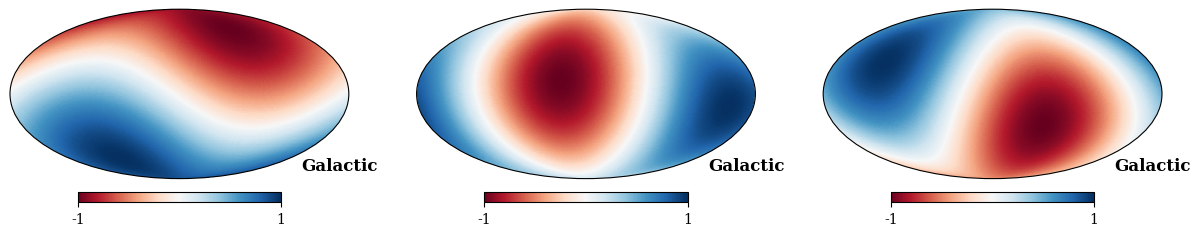
\includegraphics[width=\textwidth]{images/dipole_templates.png}
    \caption{The three orthogonal dipole templates, $D_j(\theta,\phi)$, in Galactic coordinates using a Mollweide projection, used in the least-squares fit to measure the dipole vector $\vec{\mathcal{D}}$ in the quasar catalogs.}
    \label{fig:dipole_templates}
\end{figure}

\subsection{Relationship between $|\vec{\mathcal{D}}|$ and $C_1$}

Existing literature typically describes the sky dipole using one of two conventions.
The convention used in Section \ref{sec:dipole_model} is adopted by \citet{secrest_test_2021}.
There is a direct transformation between this dipole amplitude $|\vec{\mathcal{D}}|$ and the $\ell=1$ mode of the angular power spectrum $C(\ell)$:
\begin{equation}
    C_1 = \frac{4\pi}{9}|\vec{\mathcal{D}}|^2
\end{equation}
with the specific components related to the spherical harmonic coefficients as
\begin{equation}
    \mathcal{D}_{(x,y,z)} = \sqrt{\frac{3}{4\pi}}\,a_{1(-1,0,1)}
\end{equation}
\abby{Hogg: what's the best way to write this math? \citet{gibelyou_dipoles_2012} aligns the dipole in the positive $z$ direction and then only expresses this relationship in terms of $|\vec{\mathcal{D}}|$ and $a_{10}$, without loss of generality. this is definitely the easiest to write, but it's a bit removed from what we do in practice (we use galactic coordinates and so do have to transform all three dipole components).}

\begin{figure}
    \centering
    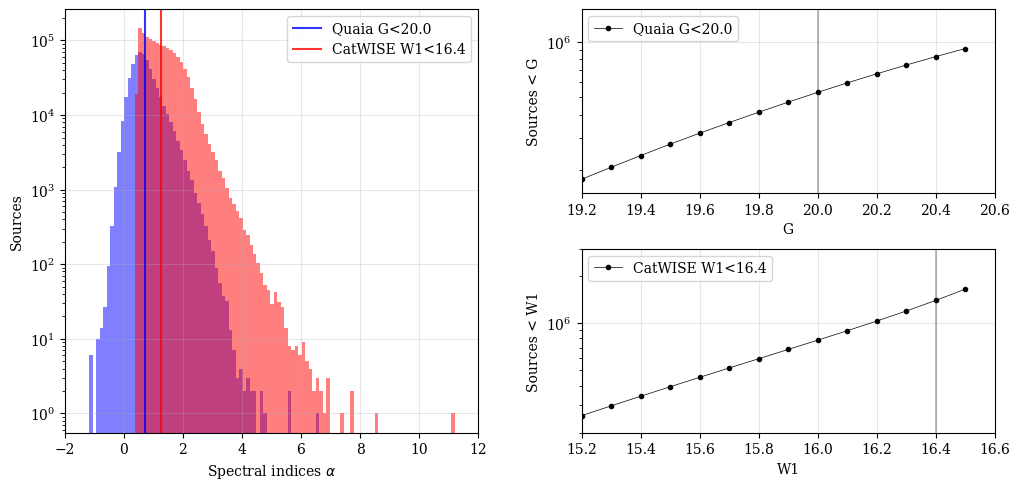
\includegraphics[width=\textwidth]{images/alphas_xs_G20.5.png}
    \caption{The spectral indices $\alpha$ and number-count slopes $x$ used to calculate the expected dipole amplitude for the \quaia and S21 fiducial samples. \textit{Left:} Histogram of the spectral indices $\alpha$ calculated for each source in the \quaia (blue) and S21 (red) fiducial samples. The vertial lines indicate the mean ($\bar\alpha=$0.71 and 1.26, respectively), which is taken as the effective value and used in Eq. \ref{eq:ellisbaldwin}. Note the sharp minimum cutoff in S21 due to the $W1-W2$ color cut made when constructing the sample. \textit{Right:} Number of sources as a function of the magnitude limit in the \quaia (top) and S21 (bottom) samples. The slope of the curve ($x=$1.30 and 1.75, respectively) at the magnitude limit of the fiducial sample, indicated by the grey vertical lines, is the number-count slope used in Eq. \ref{eq:ellisbaldwin}.}
    \label{fig:alphas_xs}
\end{figure}

\section{Dipole measurement}

\subsection{Linear least-squares fit}
\label{sec:standard_dipole}

The [most straightforward / simplest] way to measure the dipole involves a linear least-squares fit to the three orthogonal dipole templates (Figure \ref{fig:dipole_templates}).
We use the model given by Eq. \ref{eq:dipole_model}, so the four free parameters are the monopole and the amplitudes of the three dipole components:
\begin{equation}
    \vec{\theta} = [\,\bar n, d_1, d_2, d_3\,]
\end{equation}

For some choice of $\theta$, the total squared error for a healpixel $p$ centered on $(\theta_p,\phi_p)$ is
\begin{equation}
\label{eq:chisq}
    \chi^2 = \sum_p \frac{\left(n_p - n'(\theta_p,\phi_p)\right)^2}{\sigma_p^2}
\end{equation}
where $n_p$ is the observed number of quasars in the healpixel, $n'(\theta_p,\phi_p)$ is the number of quasars predicted by the model, and $\sigma_p^2$ is the [variance] \abby{Hogg: in practice we use the completeness... is this different than the \textit{variance} of the quasars in the pixel? should I call this the uncertainty squared and say that we treat the completeness as a measure of our uncertainty in that pixel?}
The best-fit \abby{I know this is a loaded term, not sure if I should expand on our definition of ``best-fit"} values of $\vec\theta$ are those which minimize $\chi^2$.
\abby{Hogg: should I write out the linear algebra for the least-squares fit ?}

S21 measures the dipole in the \catwisetwentytwenty sample (Figure \ref{fig:S21_map}) using the \texttt{healpy.fit\_dipole()} function, which performs this fit, assuming the identity for the variances $\sigma_p^2$.

\subsection{Field-level inference}
\label{sec:FLI}
\abby{or: Hogg: Simulation-based inference; Forward-modeling approach...?}

We use a forward-modeling approach to perform field-level inference, [getting/learning/recovering] posterior probability distributions over the dipole and any excess angular power that may be present in the quasar catalogs.
In particular, we employ Approximate Bayesian Computation (ABC), a likelihood-free parameter inference method, implemented using the \texttt{pyABC} package \citep{schalte_pyabc_2022}.
\texttt{pyABC} uses a sequential Monte-Carlo (SMC) scheme to iteratively update the posterior probability distribution.
The primary requisites for ABC-SMC are an executable forward-process model, a prior distribution for each parameter, a choice of distance metric, and a few hyperparameters.

We model the quasar density at a sky position $(\theta,\phi)$ as a stochastic function with two free parameters: the kinematic dipole amplitude $\dipamp$ and the level of excess angular power $\bar C$.
We assume that the kinematic dipole points in the same direction as the CMB dipole, $(\ell,b)=(264^\circ,48^\circ)$, with some amplitude $|\vec{\mathcal{D}}_k|$.
The model also has the freedom to be anisotropic at the largest angular scales, $1\le\ell\le 8$, with excess angular power which is flat in $C(\ell)$ space.
The spherical harmonic coefficients $a_{\ell m}$ are drawn stochastically from a Gaussian whose width depends on $\bar C$.
The model is called on a healpixel grid, and the kinematic dipole map $\mathcal{D}_k(\theta,\phi)$ and excess power map $\gamma(\bar C)(\theta,\phi)$ are constructed in overdensity space, so their average over all pixels is zero.
\abby{how do we feel about $\gamma$ as the excess power map?... not sure I'm a fan but not sure if there is an existing convention for this}

To convert from overdensity to quasar counts, we take
\begin{equation}
    \lambda(\theta,\phi) = (1 + \mathcal{D}_k(\theta,\phi) + \gamma(\bar C)(\theta, \phi)) \cdot \rho
\end{equation}
where $\rho$ is the quasar base rate \abby{need to explain this}, $\mathcal{D}_k(\theta,\phi)$ is the kinematic dipole contribution to the overdensity, and $\gamma(\bar C)(\theta,\phi)$ is the excess angular power contribution to the overdensity at angle $(\theta,\phi)$ on the sky.
Note that the total dipole in the map is the sum of the kinematic dipole and the ``excess power" dipole,
\begin{equation}
    \vec{\mathcal{D}}_\mathrm{tot}=\vec{\mathcal{D}}_k + \vec{\mathcal{D}}_\gamma 
\end{equation}

The map $\lambda(\theta,\phi)$ returns the number of quasars observed in a healpixel centered at $(\theta,\phi)$ in the absence of shot noise and selection effects.
To incorporate these observational effects, we multiply the map by the selection function (Section \ref{sec:selfuncs}) and draw the final quasar counts in each pixel from a Poisson distribution with expectation $\lambda(\theta,\phi)$.
An example mock generated using this model is shown in Figure \ref{fig:example_mock}.

To infer the free parameters $\dipamp$ and $\bar C$, we call the model many times, each time with the two parameters sampled at random from the prior.
The goal is to accept mocks that look like the data and reject the others, keeping track of the values of the parameters used to generate the accepted mocks.
Quantitatively, for ABC, this means condensing each mock into some summary statistic, then comparing the summary statistics of the mock and the observed data via a chosen distance metric.
We generate the mock quasar maps at $\nside=64$, and the summary statistic is the overdensity map downgraded to $\nside=1$, as the lower resolution allows for faster convergence.
The distance metric is the Euclidean distance between the mock map and the observed data map,
\begin{equation}
    \delta_i = \sqrt{\vec d_\mathrm{sim}(\theta_i)-\vec d_\mathrm{data}}
\end{equation}
where each $\vec d$ is a 16-vector of the quasar overdensity in each healpixel, and $\theta_i=\{\dipamp,\bar C\}$ are the parameters used to generate mock $i$.
The mock is accepted if $\delta_i$ is below some acceptance threshold $\varepsilon$, and rejected otherwise.

\begin{figure}
    \centering
    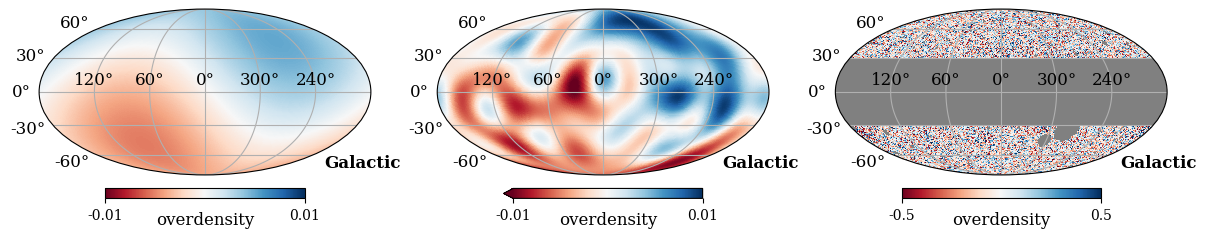
\includegraphics[width=\textwidth]{images/example_mock.png}
    \caption{Example mock \quaia-like quasar overdensity map constructed using our model, in Galactic coordinates. \textit{Left:} Kinematic dipole in the CMB dipole direction with expected amplitude 0.0052 from the Ellis-Baldwin formula (Eq. \ref{eq:ellisbaldwin}). \textit{Center:} Sum of the kinematic dipole and excess power maps. The excess power amplitude is $\bar C = 10^{-6}$, which is around \quaia shot noise, and injected at scales $1\le\ell\le 8$. \textit{Right:} Final mock overdensity map: The sum of the kinematic dipole and excess power overdensity maps, masked and Poisson-sampled to include shot noise.}
    \label{fig:example_mock}
\end{figure}


\section{Results}
\label{sec:results}

\subsection{Standard dipole measurement}
\label{sec:standard_results}


\subsection{Field-level inference}
\label{sec:fbi_results}
We use the ABC-SMC algorithm with the forward-process model described in Section \ref{sec:FLI} to infer both $|\vec{\mathcal{D}}_{\mathrm{proj},k}|$, the amplitude of the quasar dipole projected along the CMB dipole direction, and $\bar C$, the average excess angular power at $1\le\ell\le 8$.
We require 500 accepted samples per generation and run for 18 generations.
The resulting posteriors are shown in Figure \ref{fig:quaia_posterior} for \quaia and Figure \ref{fig:catwise_posterior} for \catwise.
\abby{KSF/Hogg: do we want to show any $C(\ell)$ plots here?}

\begin{figure}
    \centering
    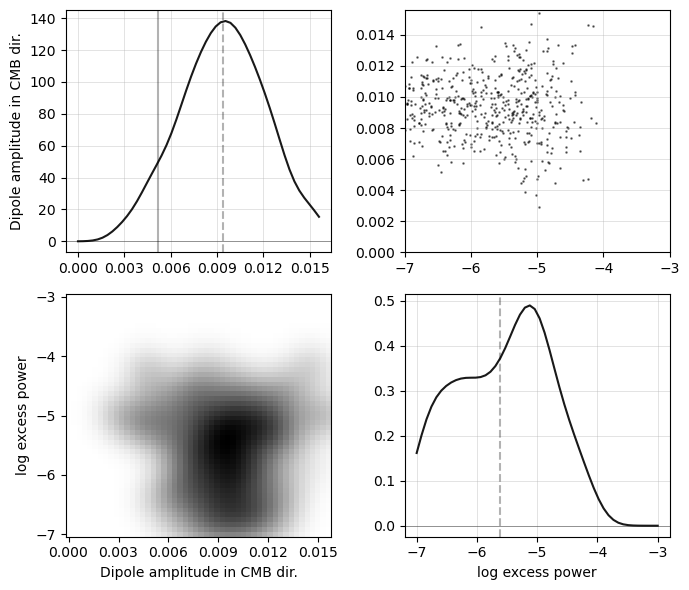
\includegraphics[width=0.6\linewidth]{images/quaia_posterior.png}
    \caption{Posterior distribution for the \quaia $G\le 20.0$ sample. The vertical solid line indicates the expected dipole amplitude from the Ellis-Baldwin test (0.0052), while the vertical dashed lines indicate the median of the parameters used to generate the accepted samples.}
    \label{fig:quaia_posterior}
\end{figure}

\begin{figure}
    \centering
    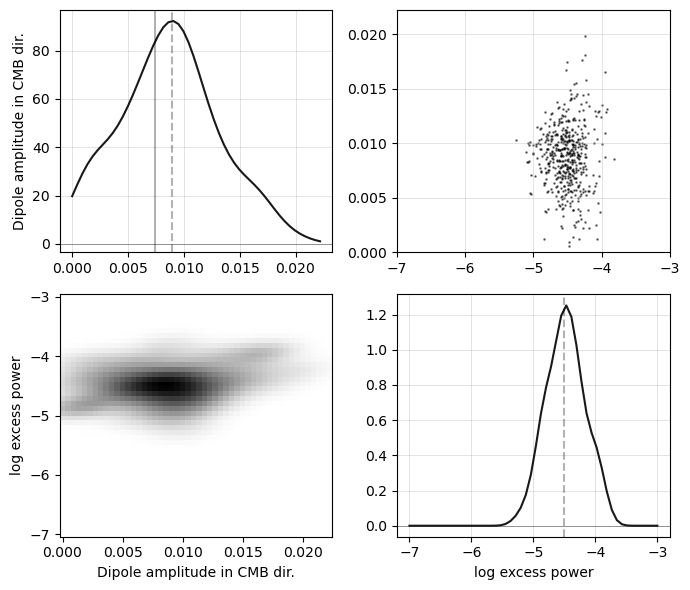
\includegraphics[width=0.6\linewidth]{images/catwise_posterior.png}
    \caption{Posterior distribution for the \catwise sample. The vertical solid line indicates the expected dipole amplitude from the Ellis-Baldwin test (0.0074), while the vertical dashed lines indicate the median of the parameters used to generate the accepted samples.}
    \label{fig:catwise_posterior}
\end{figure}


\section{All the other stuff we did}
\label{sec:additional_tests}
\begin{itemize}
    \item Infer map parameters by matching mock and data angular power spectra, $C(\ell)$: we continually ran into regularization conundrums
    \begin{itemize}
        \item tried a few ways to choose a reasonable regularization strength $\Lambda$... to no avail
    \end{itemize}
    \item Test dependence of measured dipole on sample construction choices: we found the measured dipole to be sensitive to these choices, especially the galactic plane cut (maybe not enough to match the dipole to its expectation, but definitely enough to shake S21's $4.9\sigma$ confidence)
    \begin{itemize}
        \item Galactic plane cut
        \item Magnitude cut
        \item ``Small masks" radius
        \item For \catwise, extinction correction parameters
    \end{itemize}
\end{itemize}


\section{Discussion}
\label{sec:discussion}

\appendix{Key points before I forget}
\begin{enumerate}
    \item \textit{this is not a precise measurement!!!}
    \begin{enumerate}
        \item the expected dipole amplitude is an approximation
        \item we know to expect some level of shot noise and cosmological dipole, so we don't even expect the measured dipole in these catalogs to be the kinematic dipole even in the absence of anomalous power (see Cheng et al. paper 2023)
    \end{enumerate}
    \item (connected to above point) we can't make a [robust/principled/accurate/correct] choice of regularization strength since we don't have a noise model. we can see this in our mock results
    \begin{enumerate}
        \item is it possible to have a ``correct'' choice of regularization $\Lambda$? does it depend which $\ell$ we care about? my current understanding is that if there is excess power on multiple angular scales, there is not a single choice of $\Lambda$ that can correctly recover the power at each scale $\ell$ (maybe unless we're in the unique case where the excess power $C(\ell)$ projects onto the sky mask in such a way that a single value of $\Lambda$ correctly accounts for the impact of the non-orthogonalities of the spherical harmonics)
    \end{enumerate}
\end{enumerate}

\bibliography{references}

\end{document}